\section{Experimental setup}

\subsection{Data retrieval}

In this project, it is analyzed a specific cell line, HEK293, in order
to predict the activation of promoters and enhancers. We consider a set
of regions of the human genome, 200 nucleotide long. Each region
corresponds to a CRE (promoter or enhancer), which may be active or not,
and it is characterized by both sequence and epigenomic data. In detail,
the sequence data is simply the nucleotide sequence and the epigenomic
data refers to the level of interaction between the region and proteins.
Starting from the epigenomic data, they come from the
\href{https://www.encodeproject.org/}{ENCODE} project and the data
considered are obtained by the ChiP-sequencing technique. The labels of
our data, that say if a region is active or inactive, are taken from
FANTOM, which contains a wide collection of promoters and enhancers and
indicates if they are active or not in a specific cell line. The amount
of data obtainable from ENCODE is extremely large and they must be
queried with the FANTOM data to extract only the region considered in
this project. Fortunately, this task has been already done and the
epigenomic data of promoters and enhancers can be found in this
\href{https://github.com/LucaCappelletti94/epigenomic_dataset}{repository},
which offers also a python package to automatically download and use
these data. The sequence data instead requires the genome sequence of
the cell line, obtainable from
\href{https://genome.ucsc.edu/index.html}{UCSC Genome Browser} with this
python
\href{https://github.com/LucaCappelletti94/ucsc_genomes_downloader}{utility},
which can be filtering in order to obtain only the nucleotide sequences
of promoters and enhancers.

\subsection{Data preprocessing}

\subsubsection{Epigenomic data}

The dataset obtained has to be processed to remove wrong values and make
data easier to analyze. It is important to specify that only the
epigenomic features are preprocessed. In particular, the data are
modified through the following operations:

\begin{itemize}
\item
  \textbf{NaN values substitution:} in biology experiments, there are
  some practical cases where some data could be NaN. This situation,
  especially when the NaN values are many, is dangerous for the learning
  model. If it happens, there are a lot of different techniques to fix
  it. If there NaN values are concentrated in a single sample or in a
  single feature it is convenient to remove it. Otherwise, if the NaN
  values are scattered in all dataset, they could be replaced by
  empirical values, like the mean or the median. In the dataset used in
  this project, there are only one NaN value in the enhancers epigenomic
  data and no one for the promoters. This single NaN value has been
  replaced with the median.
\item
  \textbf{Constant feature elimination:} in some dataset could be
  features with the same value for each sample. This situation doesn't
  help the learning machine and the these features can be removed. This
  is not the case of the data used in this project. every features has
  different values in at most one sample.
\item
  \textbf{Z-scoring:} it is a way to standardizing the data. The Z-score
  is the number of standard deviation by which the value of a raw score
  is closed to the population mean: it is positive if it is above the
  mean or it is negative otherwise. The Z-scoring is calculated by
  subtracting the average and dividing by the standard deviation. In
  this way, the new data have mean 0 and variance 1. This method has a
  problem related to the outliers and it has to be fixed by subtracting
  the median and dividing by the standard deviation between the
  interquartile range from 0.25 to 0.75. This method, applied to the
  project data, is also called Robust Scaler.
\end{itemize}

\subsubsection{Sequence data}

The sequence data are composed of a series of 200 letters of 4 different
types, one for each nucleotide. To be used by the models, these data
must be converted in numbers. To do this, it is applied to the one-not
encoding technique, which converts each letter in the sequence into four
numbers which represent the four letters. These numbers are normally 0
except the number that corresponds to the letter which is set to 1.
After this process, the initial sequences formed by 200 letters are
encoded in a series of 800 numbers.

\subsection{Data checking}

In an machine learning project, it is very important to check if the
data can effectively used by machine learning models. First of all it is
necessary to verify the sample-feature imbalance. This control aim to
verify the rate between samples and features. Having a low rate means
that the sample are few respect to the features and the learning machine
isn't able to generalize on the real data. Fortunately, this isn't the
case of this dataset, in particular the rate between sample and features
for promoters is 482 and 316 for enhancers. Another important factor ti
consider is the imbalance between the classes. In some real dataset,
especially in biology, there could be a strong imbalance between
classes. For example, if it is considered a rare disease, the positive
samples are few than the negative one and the learning machine will tend
to predict a wrong result, tending to the majority class. In these
cases, it is necessary to adopt techniques to avoid this problem. This
is not the case of this dataset because the rate between negative and
positive example is 7.68 for promoters and 8.41 for enhancers as shown
in the figure.

\begin{figure}[h!]
\centering
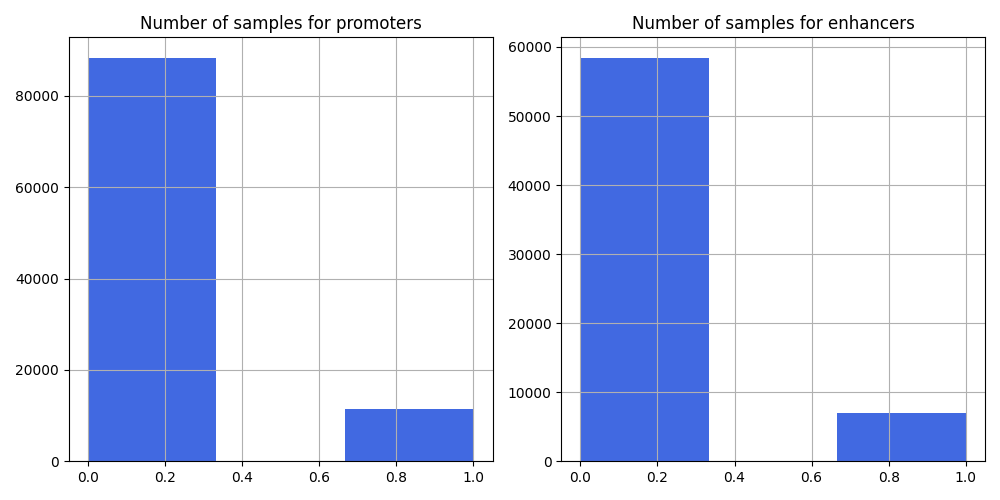
\includegraphics[width=0.7\linewidth]{../images/plot_class_imbalance.png}
\caption{Data imbalance for promoters and enhancers}
\end{figure}

\subsection{Data visualization}

\subsubsection{Data distribution}
Visualizing the data distribution is helpful to better understand the
dataset composition. Since the features are about 200 and it is
difficult and useless to represent all distributions, there were
selected and represented the 5 most different features between active
and inactive regions, both for promoters and enhancers. The histograms
below represent the Euclidean distance between the feature values, which
are filtered before 0.05 and after 0.95 percentile to reduce the impact
of the outliers. In particular, the blue and orange colors refers to
inactive and active region respectively. The first image shows the
feature distributions of promoters and the second one shows the
enhancers features distributions.

\begin{figure}[h]
\centering
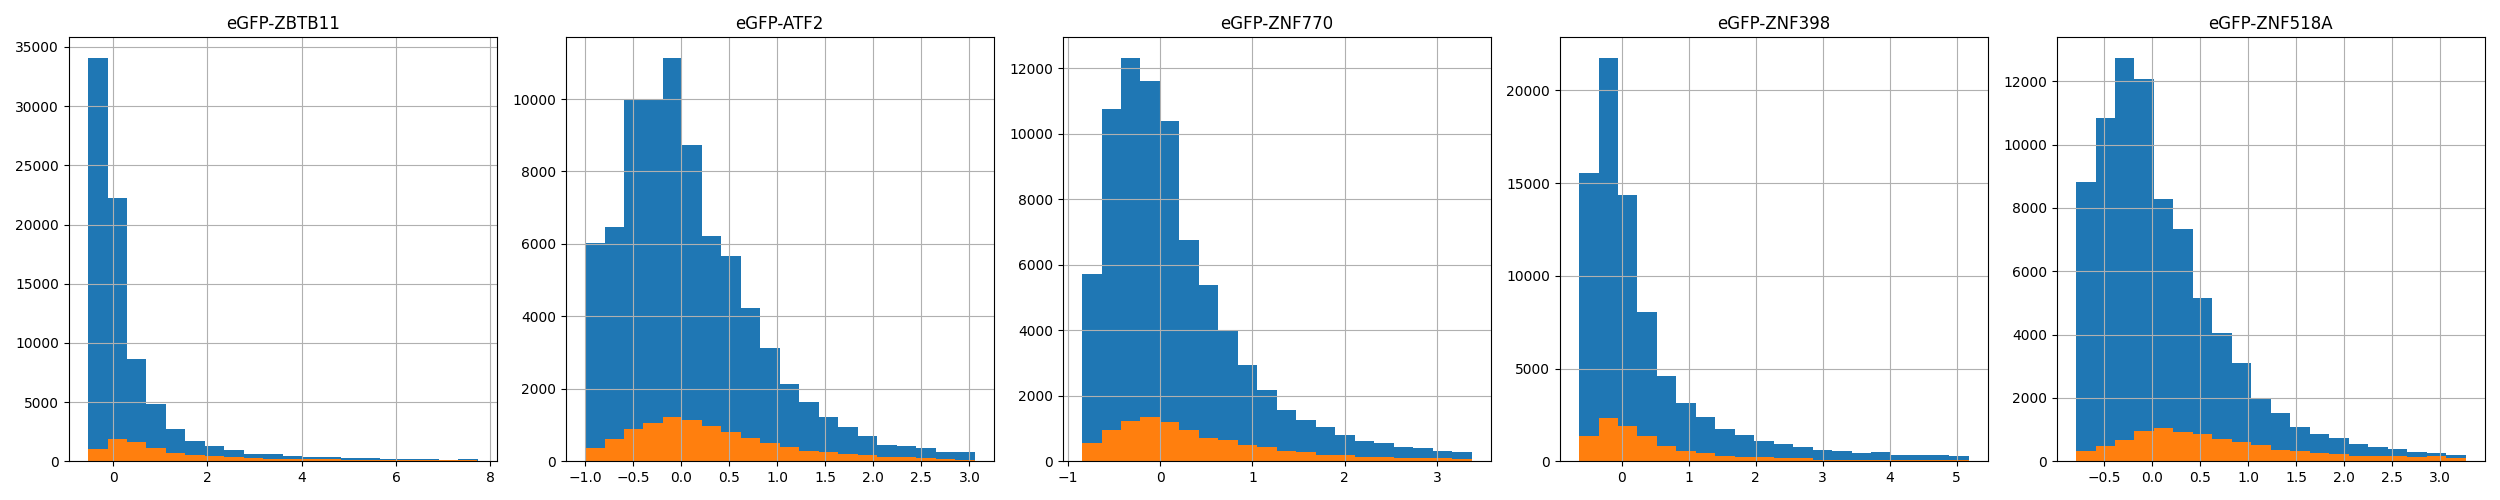
\includegraphics[width=0.95\linewidth]{../images/plot_feature_distribution_promoters.png}
\caption{Most different feature distribution of active and inactive promoters}
\end{figure}

\begin{figure}[h]
\centering
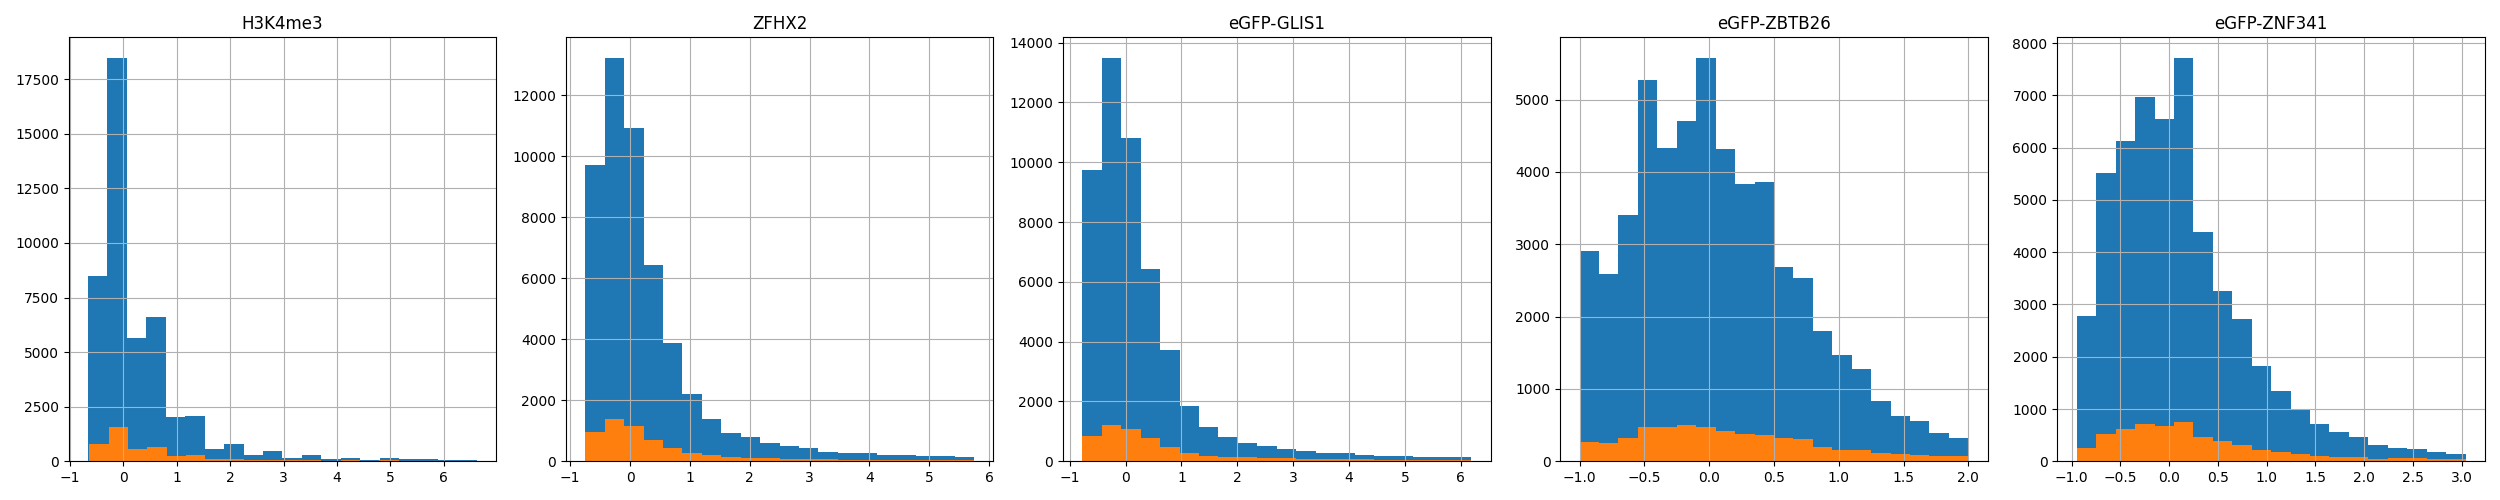
\includegraphics[width=0.95\linewidth]{../images/plot_feature_distribution_enhancers.png}
\caption{Most different feature distribution of active and inactive enhancers}
\end{figure}

Another interesting point of view is given by the visualization of the
differences between the distributions of the pairs of features. As done
in the previous method, only the 5 most different pairs of features are
considered and the values are filtered between 0.05 and 0.95. This time
the colors represent the two features and not the regions activation.

\begin{figure}[h]
\centering
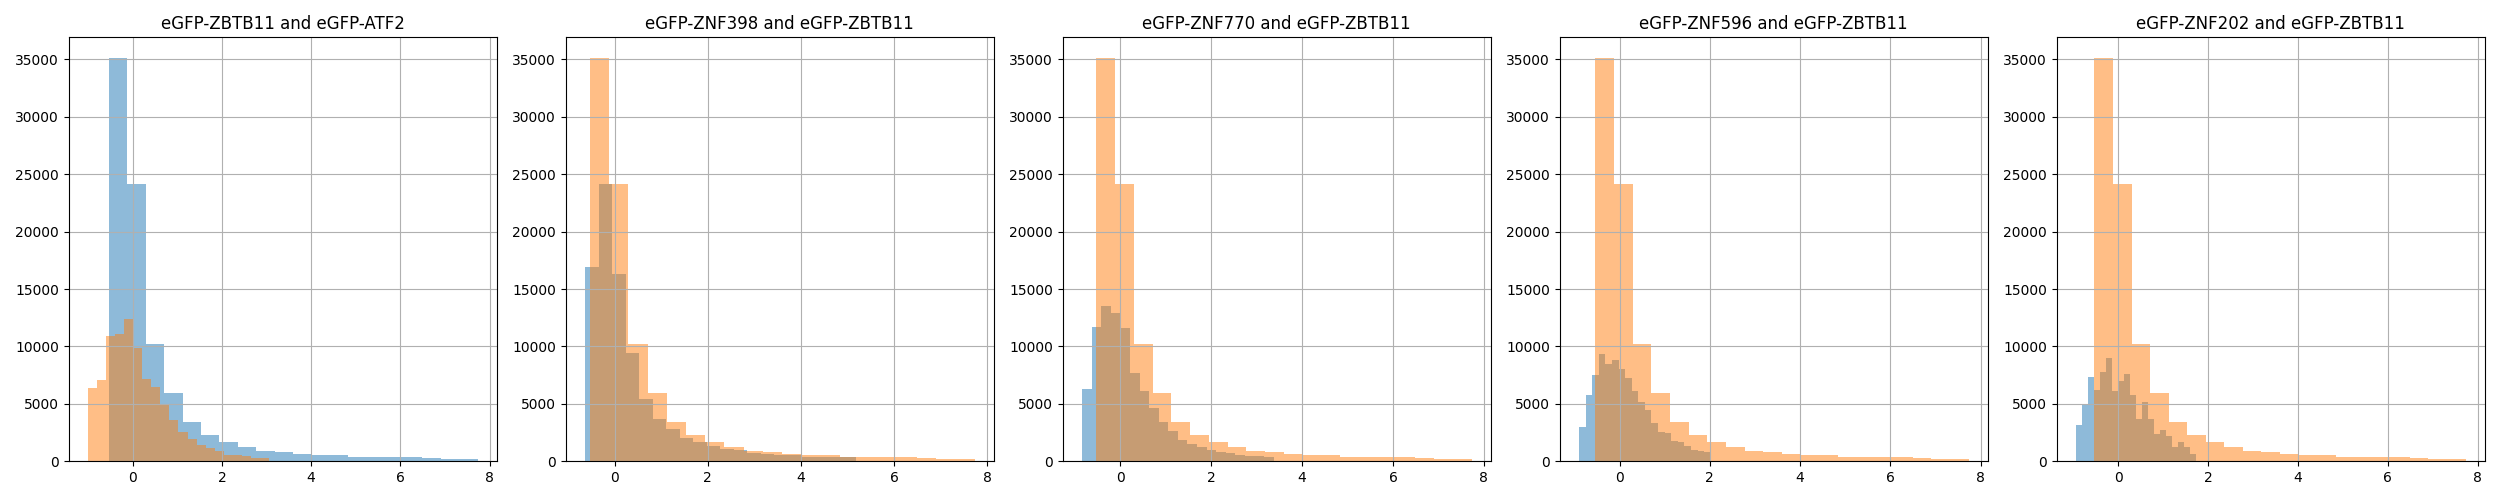
\includegraphics[width=0.95\linewidth]{../images/plot_pair_feature_promoters.png}
\caption{Most different feature distributions pair of promoters}
\end{figure}

\begin{figure}[h]
\centering
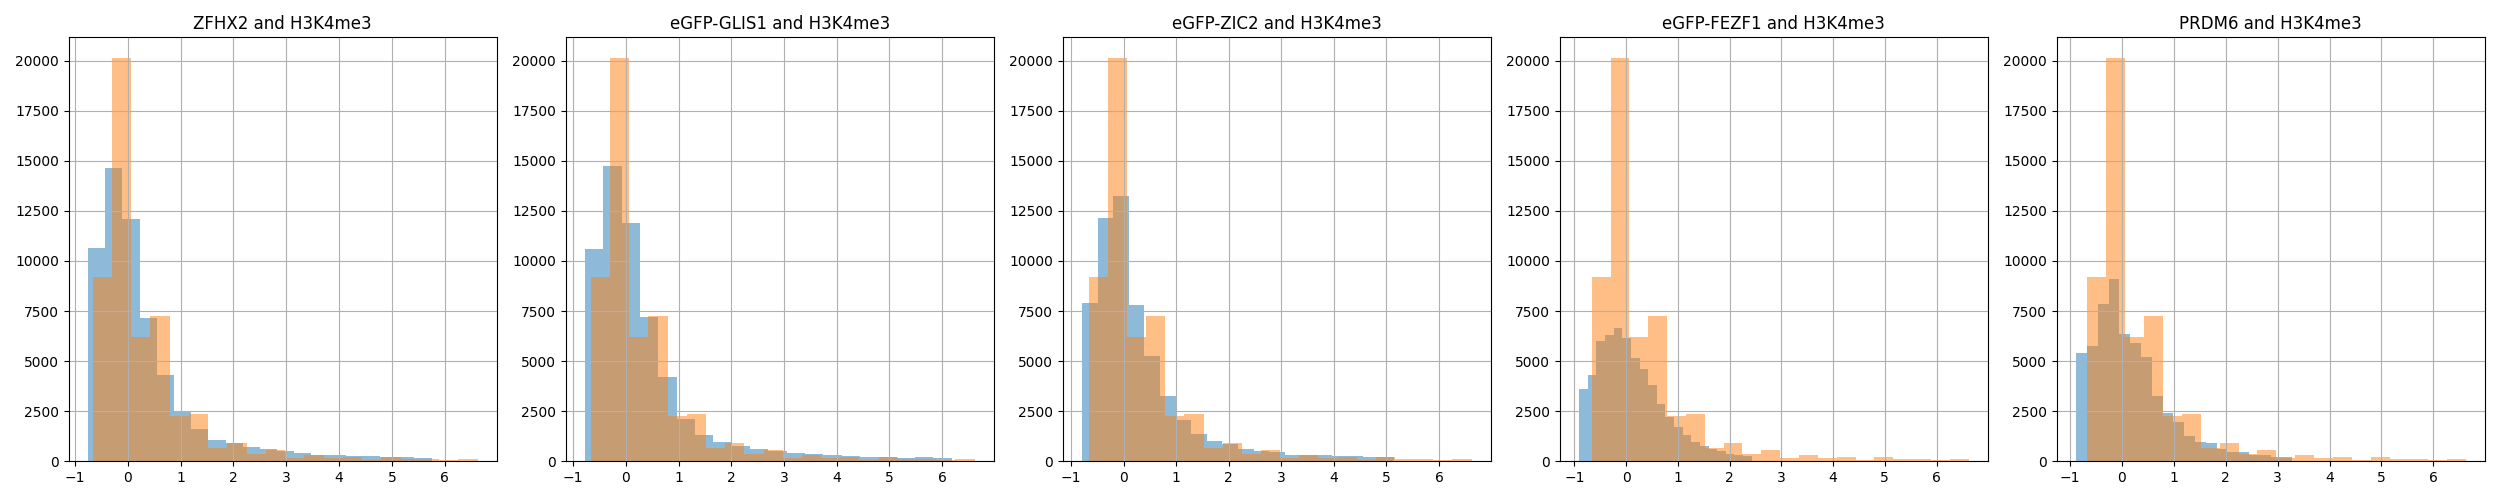
\includegraphics[width=0.95\linewidth]{../images/plot_pair_feature_enhancers.png}
\caption{Most different feature distributions pair of enhancers}
\end{figure}

\subsubsection{Data decomposition}

The data decomposition is the process through which the data
dimensionality is reduced in order to visualize the data distribution in
a 2D or 3D space. In this way the curse of dimensionality is partially
reduced. The coursed phenomena appears in a machine learning problem
when the data dimensionality increases, beacuse the volume of the space
grows and the data become sparse, invalidating any method that requires
statistical significance. In the specific domain of machine learning,
for each dimension there should be at least 5 samples for not
overfitting the model. In this case the data decomposition technique is
used only for visualization purpose.

\paragraph{PCA}

The principal component analysis (PCA) uses a simple idea: given a
collection of points in multi dimensional space, a best fitting line is
the one that minimizes the average square distance from the points to
the line. The next best-fitting line is similar but chosen from the
direction orthogonal to the first. Repeating this process produces an
orthogonal basis in which different individual dimensions of the data
are uncorrelated. These basis vectors are called principal components.
This transformation is defines as follow: the first principal component
has the largest possible variance and the succeeding components has the
highest variance under the constraint that it is orthogonal to the
previous component. It is important to specify that PCA is sensitive to
the relative scaling of the original variables: this is why it has be
run before applying the z-scoring. The figure below shows the PCA
decomposition for:

\begin{itemize}
\item
  epigenomic data of active and inactive promoters;
\item
  epigenomic data of active and inactive enhancers;
\item
  sequence data of active and inactive promoters;
\item
  sequence data of active and inactive enhancers;
\item
  sequence data of active and inactive regions (both promoters and
  enhancers);
\item
  sequence data of region types.
\end{itemize}

\begin{figure}[h]
\centering
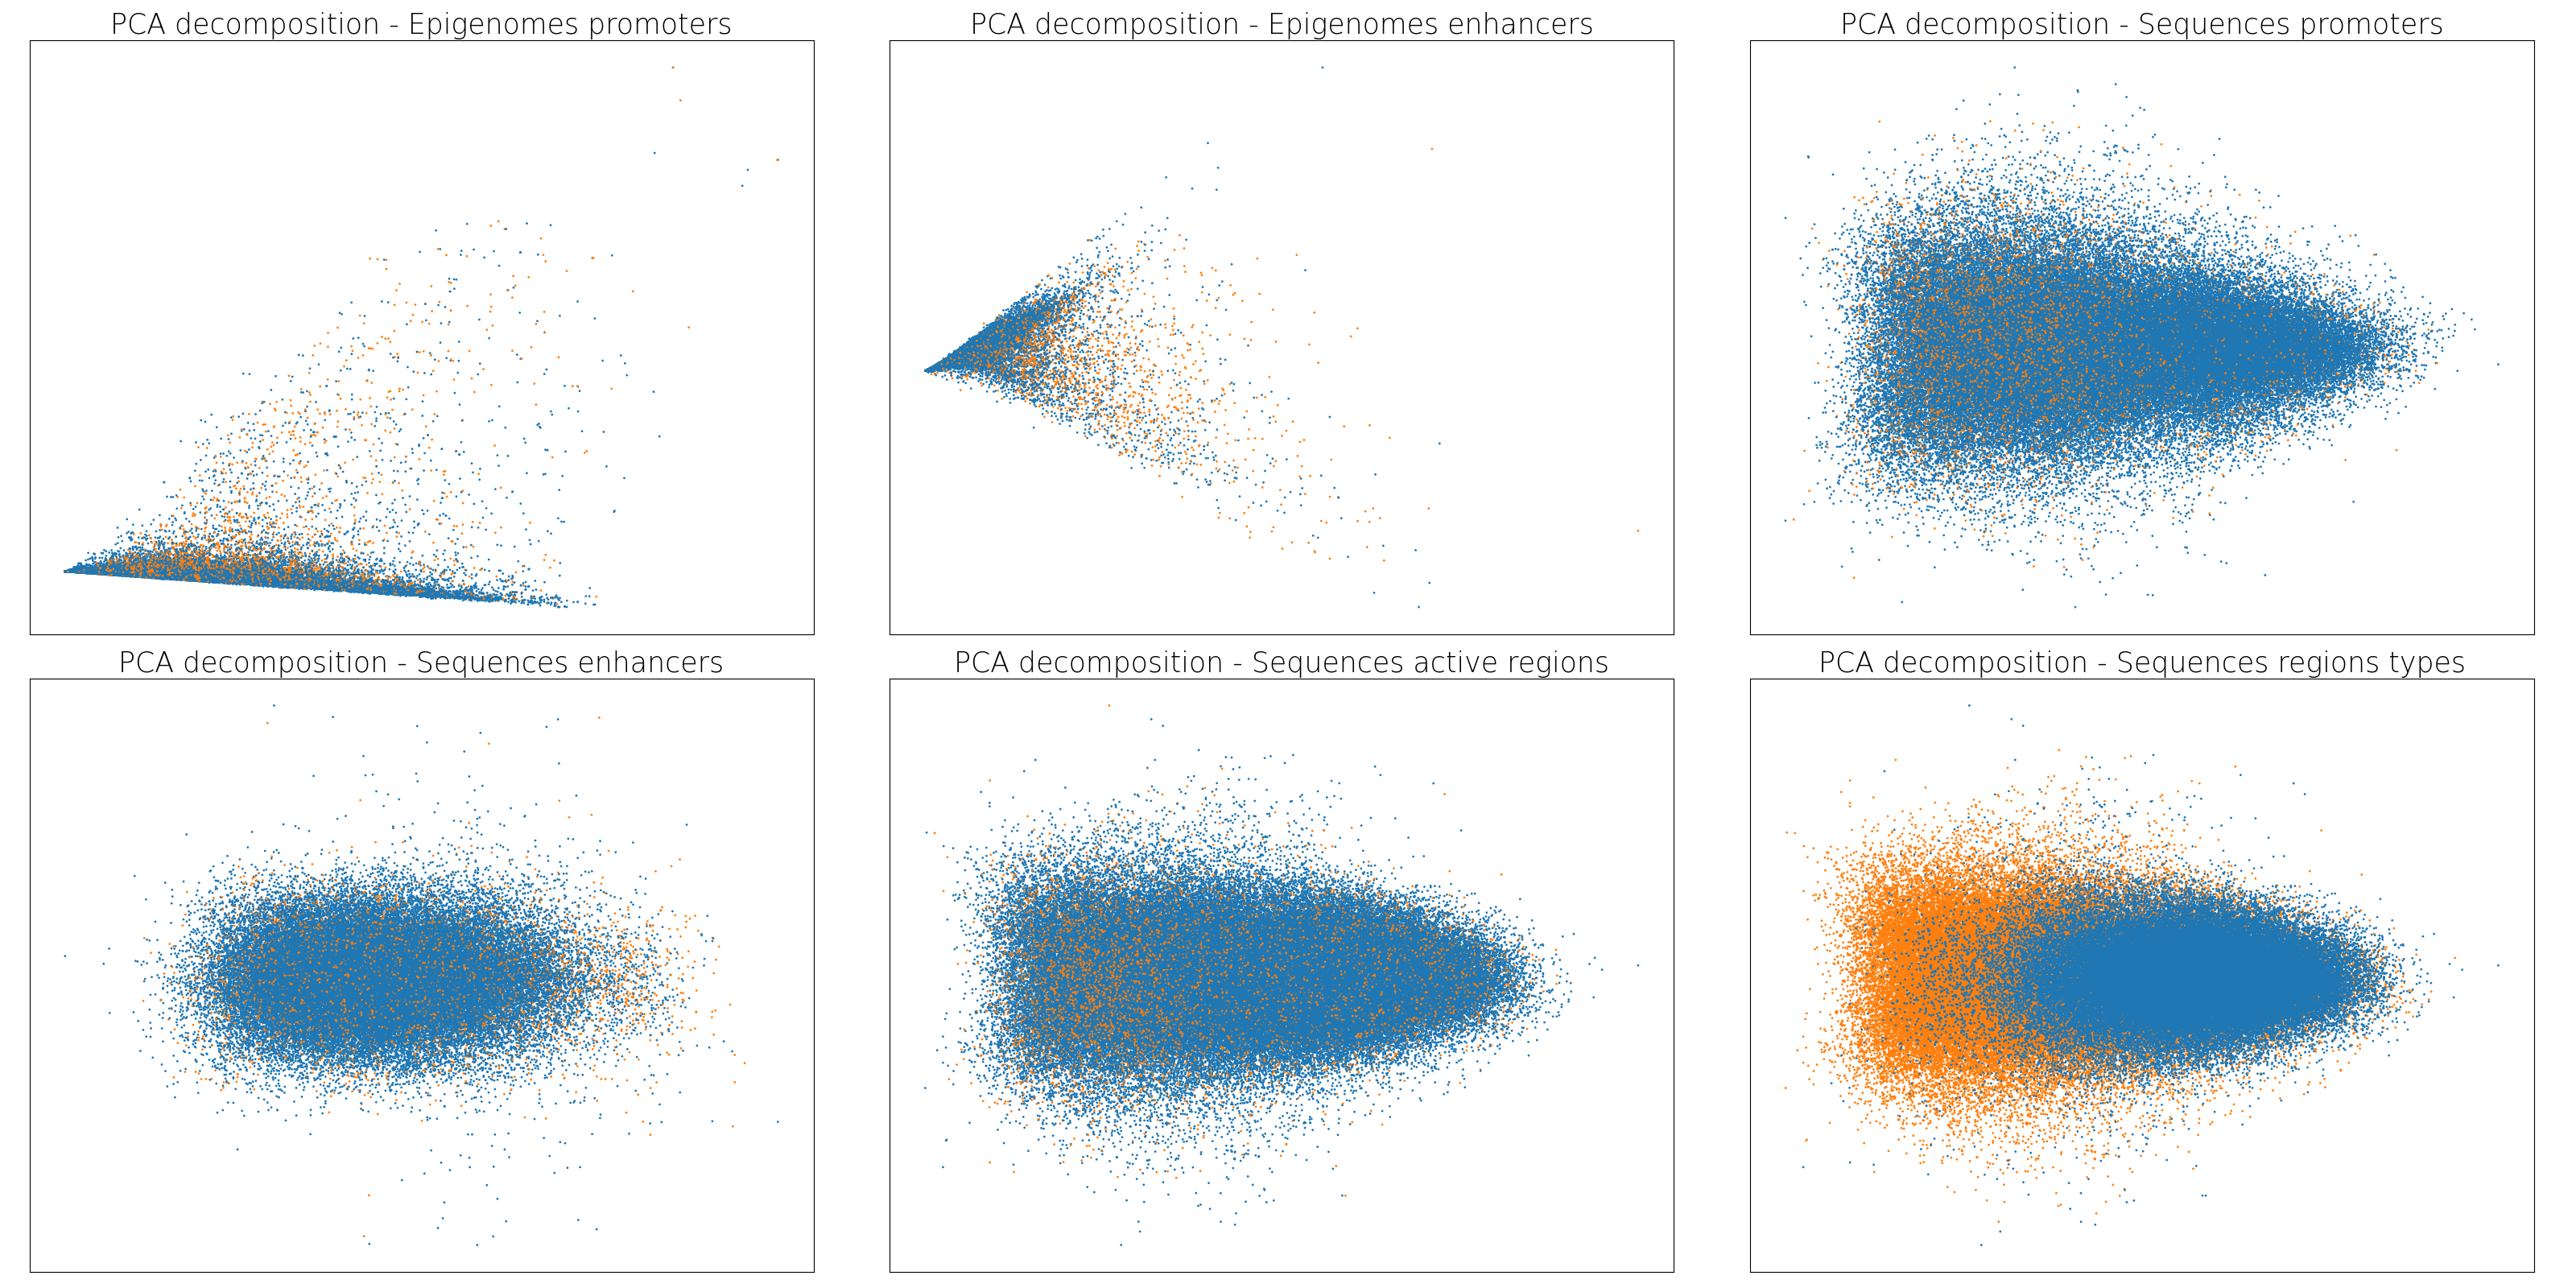
\includegraphics[width=0.95\linewidth]{../images/plot_pca.png}
\caption{PCA data decomposition}
\end{figure}

\paragraph{TSNE}

The T-distributed Stochastic Neighbor Embedding (TSNE) is an algorithm
for data visualization. It applies a nonlinear dimensionality reduction
and it is particularly effective for visualizing high-dimensionality
data in a low dimensional space of two or three dimensions.
Specifically, similar objects in high dimension are modeled by nearby
points in two or three dimensions and dissimilar objects are modeled by
distant points with high probability. In this project are used
\href{https://github.com/CannyLab/tsne-cuda}{tsne-cuda}, the state of
the art TSNE implementation which runs in GPU, developed by CannyLab of
the Berkeley university. The figure below shows the data decomposition
obtained with TSNE (set with 42 of random seed and 5000 of perplexity,
to prevent errors) for:

\begin{itemize}
\item
  epigenomic data of active and inactive promoters;
\item
  epigenomic data of active and inactive enhancers;
\item
  sequence data of active and inactive promoters;
\item
  sequence data of active and inactive enhancers;
\item
  sequence data of active and inactive regions (both promoters and
  enhancers);
\item
  sequence data of region types.
\end{itemize}

\begin{figure}[h]
\centering
\includegraphics[width=0.95\linewidth]{../images/tsne_5000.png}
\caption{TSNE data decomposition}
\end{figure}
\newpage
\subsection{Feature selection}

Since the epigenomic data has a large number of feature, it is important
to apply methods to find those features which are unnecessary or
dangerous for the learning machines and to remove them. Only he
epigenomic data are treated using this procedure, while the sequence
data are used as is. In this project, three different types of feature
selection techniques are used:

\begin{itemize}
\item
  \textbf{Check of feature-output correlation:} the feature not
  correlated with output can be removed. In particular, the Person and
  Spearman methods are used to finding monotonic and linear correlation
  respectively and, subsequently, the uncorrelated features found using
  these methods are tested with the MIC algorithm to check non-linear
  correlation with output. In the end, those features whit no
  correlation with output (bot linear and non-linear) are removed. 
\item
  \textbf{Check of feature-feature correlation:} the pairs of feature
  strongly correlated are not necessary for the learning machine,
  because they express the "same concept". In this way, in a pair of
  correlated features, the one with less entropy can be removed. In this
  project are applied the Pearson and Spearman method to check
  feature-feature monotonic correlation.
\item
  \textbf{Automatic feature selection:} the last way to remove feature
  is to test their utility for a learning machine. In particular, The
  Boruta method with a random forest is applied to the data and those
  features useless for that model have been dropped.
\end{itemize}

All these techniques are applied. The initial amount of features is 207
for promoters and enhancers. More in detail, the following pipeline is
applied for feature selection:

\begin{itemize}
\item
  Apply the Pearson method for feature-output correlation. There are
  selected 9 uncorrelated features for promoters and 28 for enhancers
  with a p\_value threshold of 0.01
\item
  Apply the Spearman method for feature-output correlation. There are
  selected 6 uncorrelated features for promoters and 27 for enhancers
  with a p\_value threshold of 0.01
\item
  The uncorrelated features found with Pearson and Spearman are not
  unique, so the two sets are unified with no repetition. The resulting
  set has 12 and 32 features for promoters and enhancers respectively
\item
  Apply the MIC method for feature-output correlation on the feature
  selected with Pearson and Spearman to check the non-linear
  correlation. After the execution, MIC find no non-linear correlation
  on the examined features with a threshold of 0.05, so there are
  removed 12 features for promoters and 32 for enhancers
\item
  Apply the Pearson method to find the feature-feature correlation. In
  this case, there are selected 0 pair of extremely correlated features
  using a p\_value threshold of 0.01 and a correlation threshold of
  0.95, so no features are removed
\item
  Apply the Spearman method to find the feature-feature correlation. In
  this case, there are selected 0 pair of extremely correlated features
  using a p\_value threshold of 0.01 and a correlation threshold of
  0.95, so no features are removed
\item
  Apply the Boruta method to remove the features useless for the random
  forest. The random forest classifier is set using the following
  parameters:

  \begin{itemize}
  \item
    n\_estimators = auto
  \item
    alpha = 0.05
  \item
    max\_iter = 10
  \item
    random\_state = 42
  \end{itemize}
\item
  After 300 iterations Boruta finds 4 useless features for promoters and
  36 for enhancers.
\item
  In the end, the total amount of features is 191 and 139 for promoters
  and enhancers respectively. In the following subsections, the features
  selection techniques are explained more in detail. 
\end{itemize}

\subsubsection{Data correlation with output}

A check which can be applied to the data is the correlation between
features and output. If a feature isn't correlated with a specific
output it is completely useless and it can be dropped. To do this, the
Pearson and Spearman tests are applied, which measure the monotonic and
linear correlations respectively. After that, the candidate
non-correlated features are tested with the MIC (Maximal information
coefficient) that tests the non-linear correlation between features and
output. Only the features found with Pearson and Spearman methods are
tested using MIC to check if they nave non-linear correlation with
output. More in detail, the Pearson correlation method measures the
linear correlation between the two datasets. In particular, the Pearson
coefficient has a value between -1 and +1, where -1 is a total negative
linear correlation, 0 implying no correlation, and +1 is a total
positive linear correlation. Instead, the Spearman correlation
coefficient doesn't require that the two datasets are normalized and it
measures the monotonicity relationship between them. The Spearman
coefficient varies between -1 and +1, like Pearson's. Now is the moment
to apply the MIC procedures to the feature selected by Pearson and
Spearman method in order to find non-linear correlations. It is
important to specify that Pearson's, Spearman's and MIC's results are
significant if they are is calculated over a large dataset, typically
with 500 samples or more. In the end, the features uncorrelated with
output can be removed.

\subsubsection{Feature correlation}

To make the data less heavy, it is possible to find and remove tightly
correlated features. The correlation can be measured using the Pearson
or MIC method. In this project, the Pearson method is used to save time
(MIC is computationally complex). When two features appear correlated,
the one with the lower entropy is removed. The entropy can be
interpreted as the average level of information or uncertainty given by
a variable. In this project, there aren't features extremely correlated
but it is interesting to examine the most correlated and least
correlated features, as shown in the images below. The first pair of
images show the most correlated and uncorrelated features in promoters
and enhancers respectively found with Pearson method. The last pair
show the two most correlated and uncorrelated features found with
Spearman method. The blue and orange colors refers to inactive and
active region respectively.

\begin{figure}[h!]
\centering
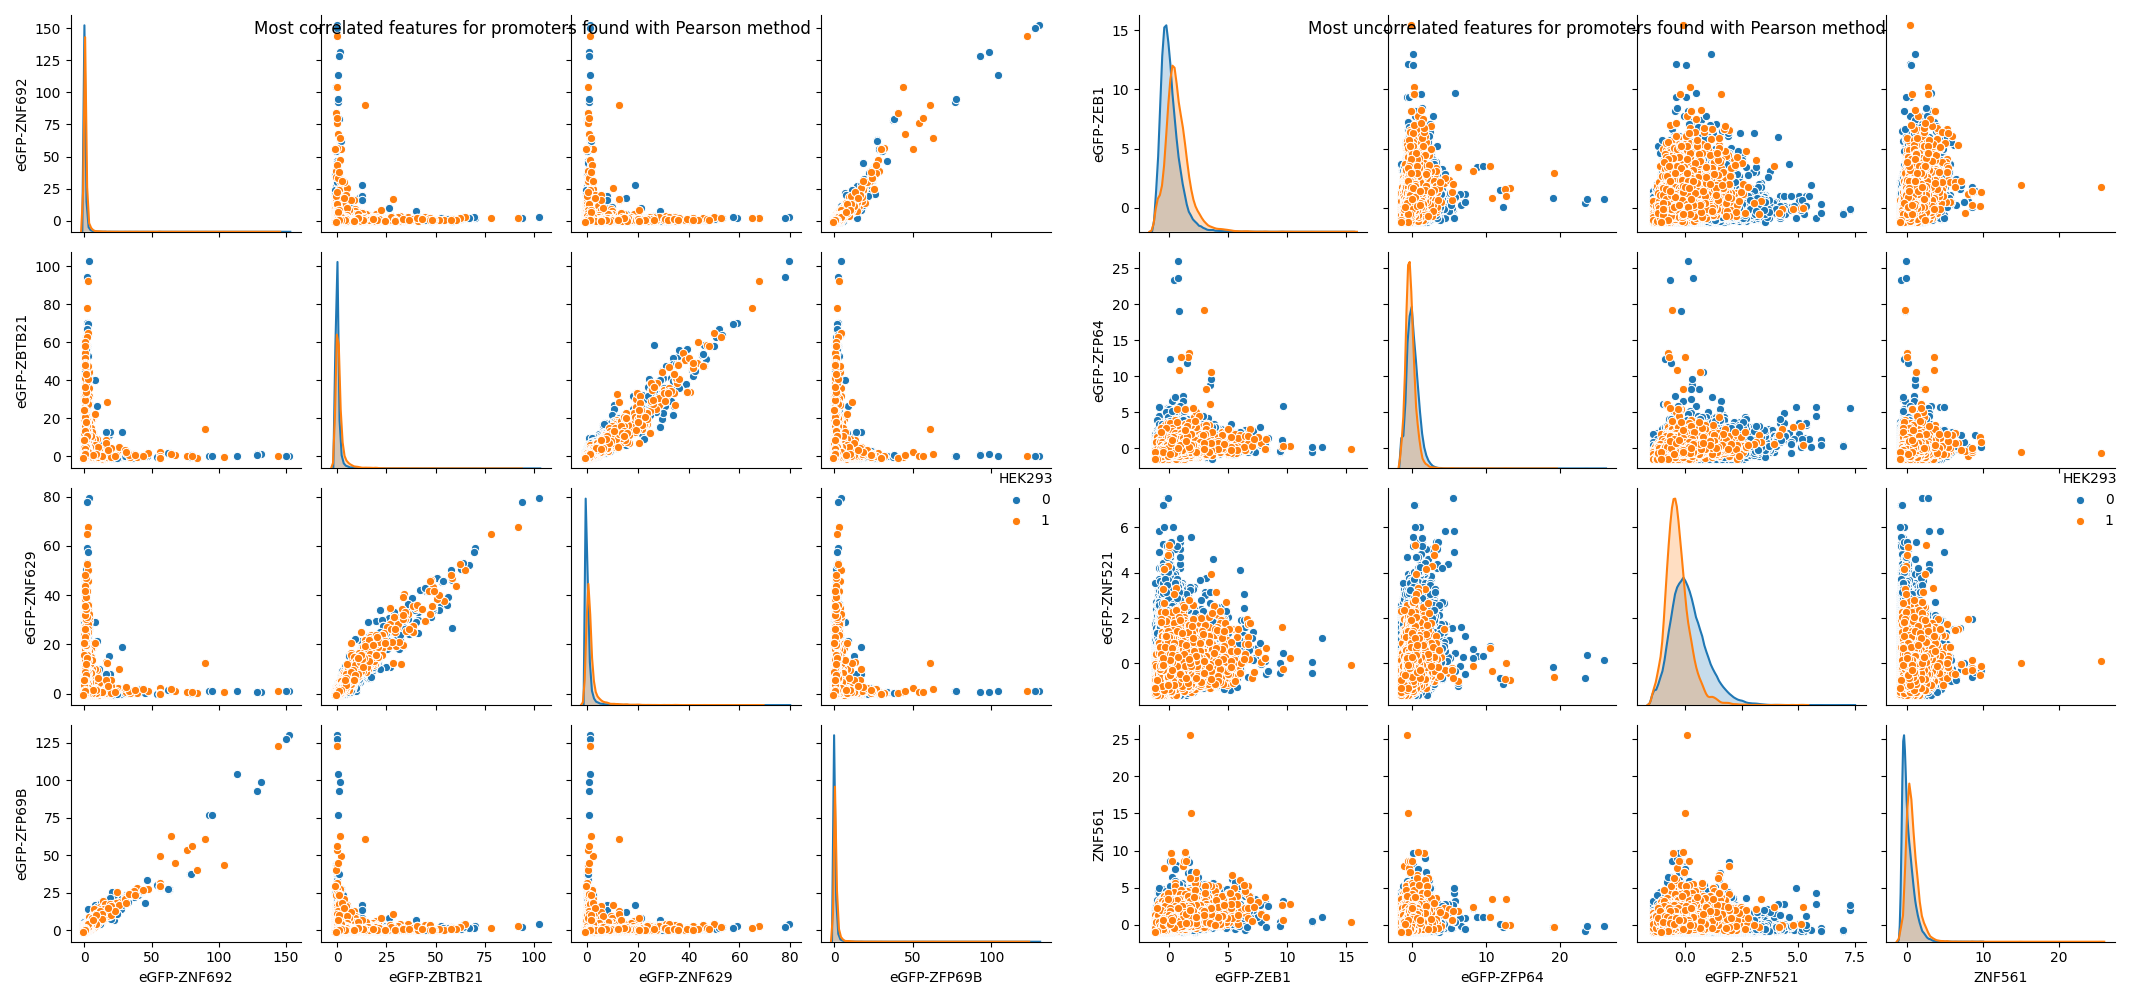
\includegraphics[width=0.98\linewidth]{../images/plot_pearson_promoters_correlated_uncorrelated.png}
\caption{Most correlated and uncorrelated feature with output for promoters found with Pearson method}
\end{figure}
\newpage
\begin{figure}[h!]
\centering
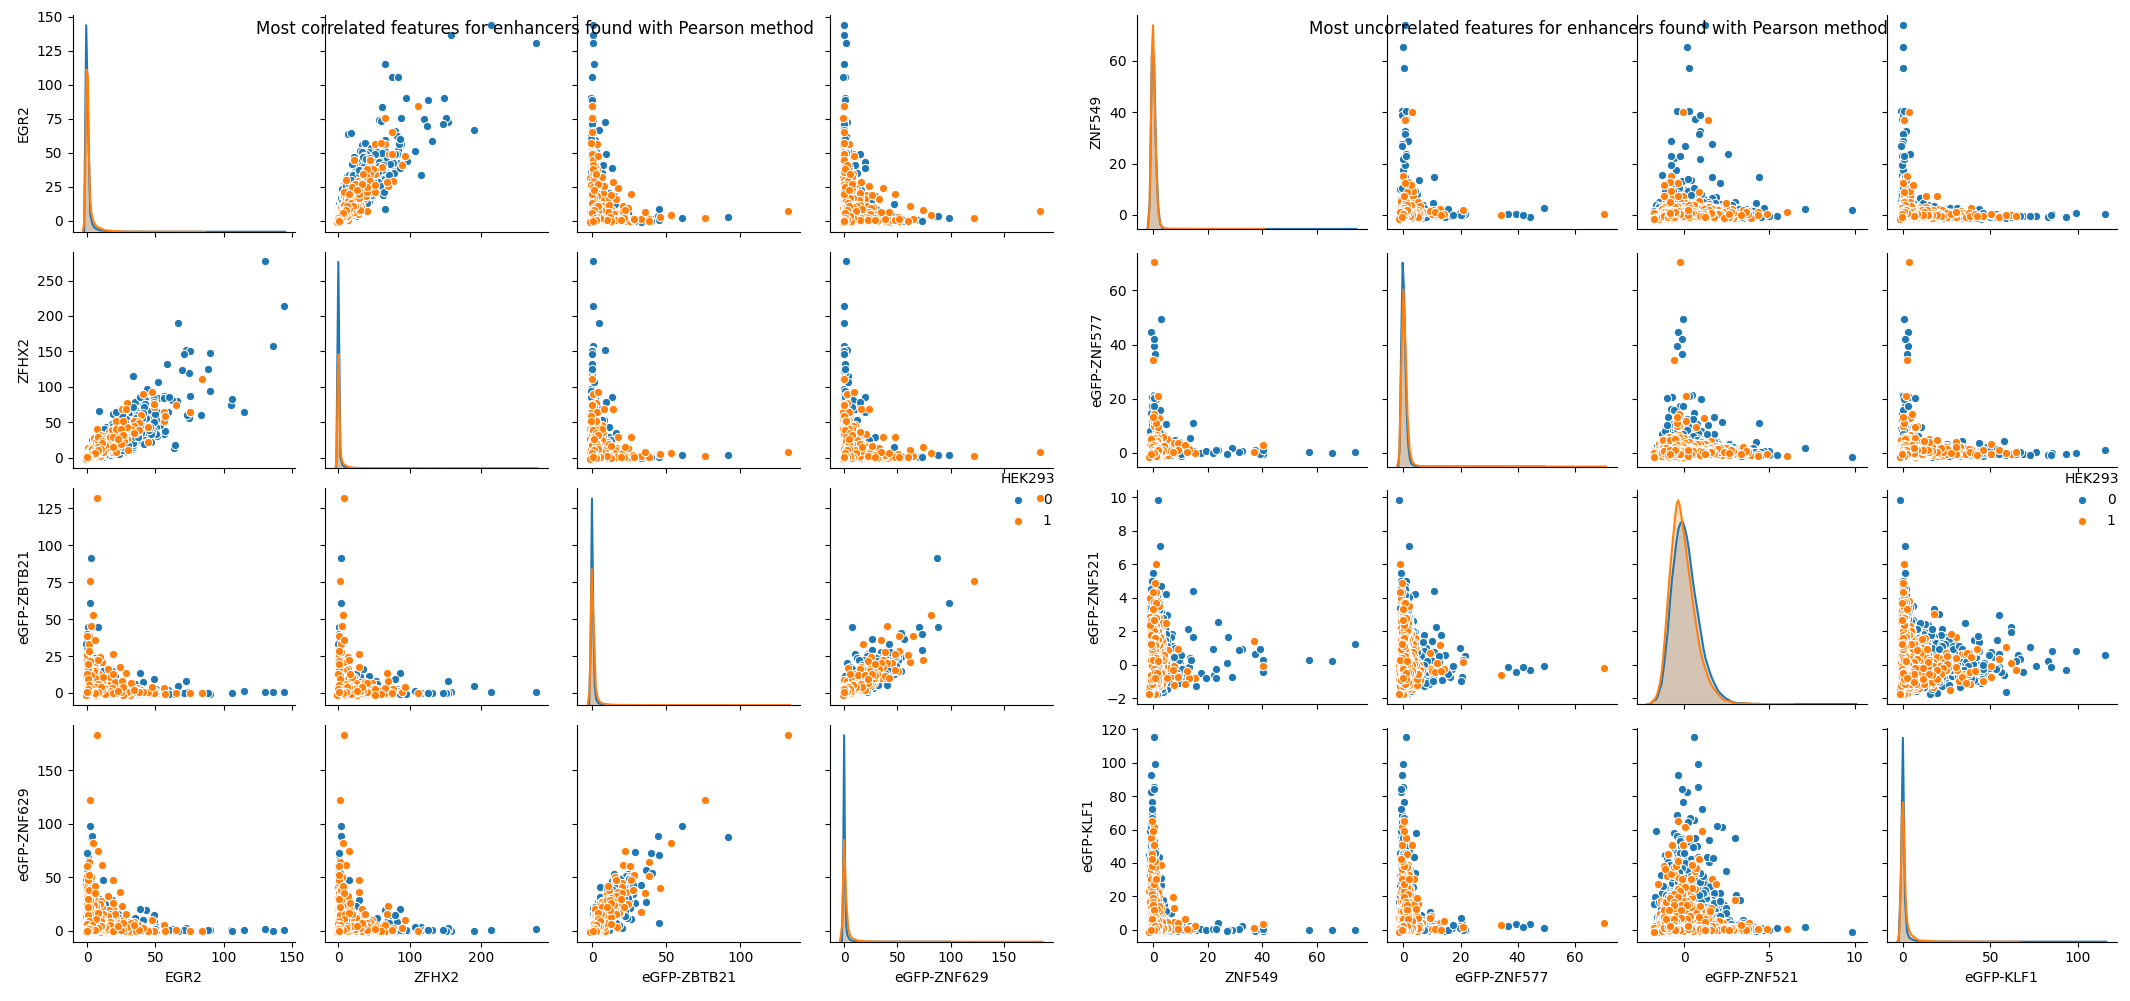
\includegraphics[width=0.98\linewidth]{../images/plot_pearson_enhancers_correlated_uncorrelated.png}
\caption{Most correlated and uncorrelated feature with output for enhancers found with Pearson method}
\end{figure}

\begin{figure}[h!]
\centering
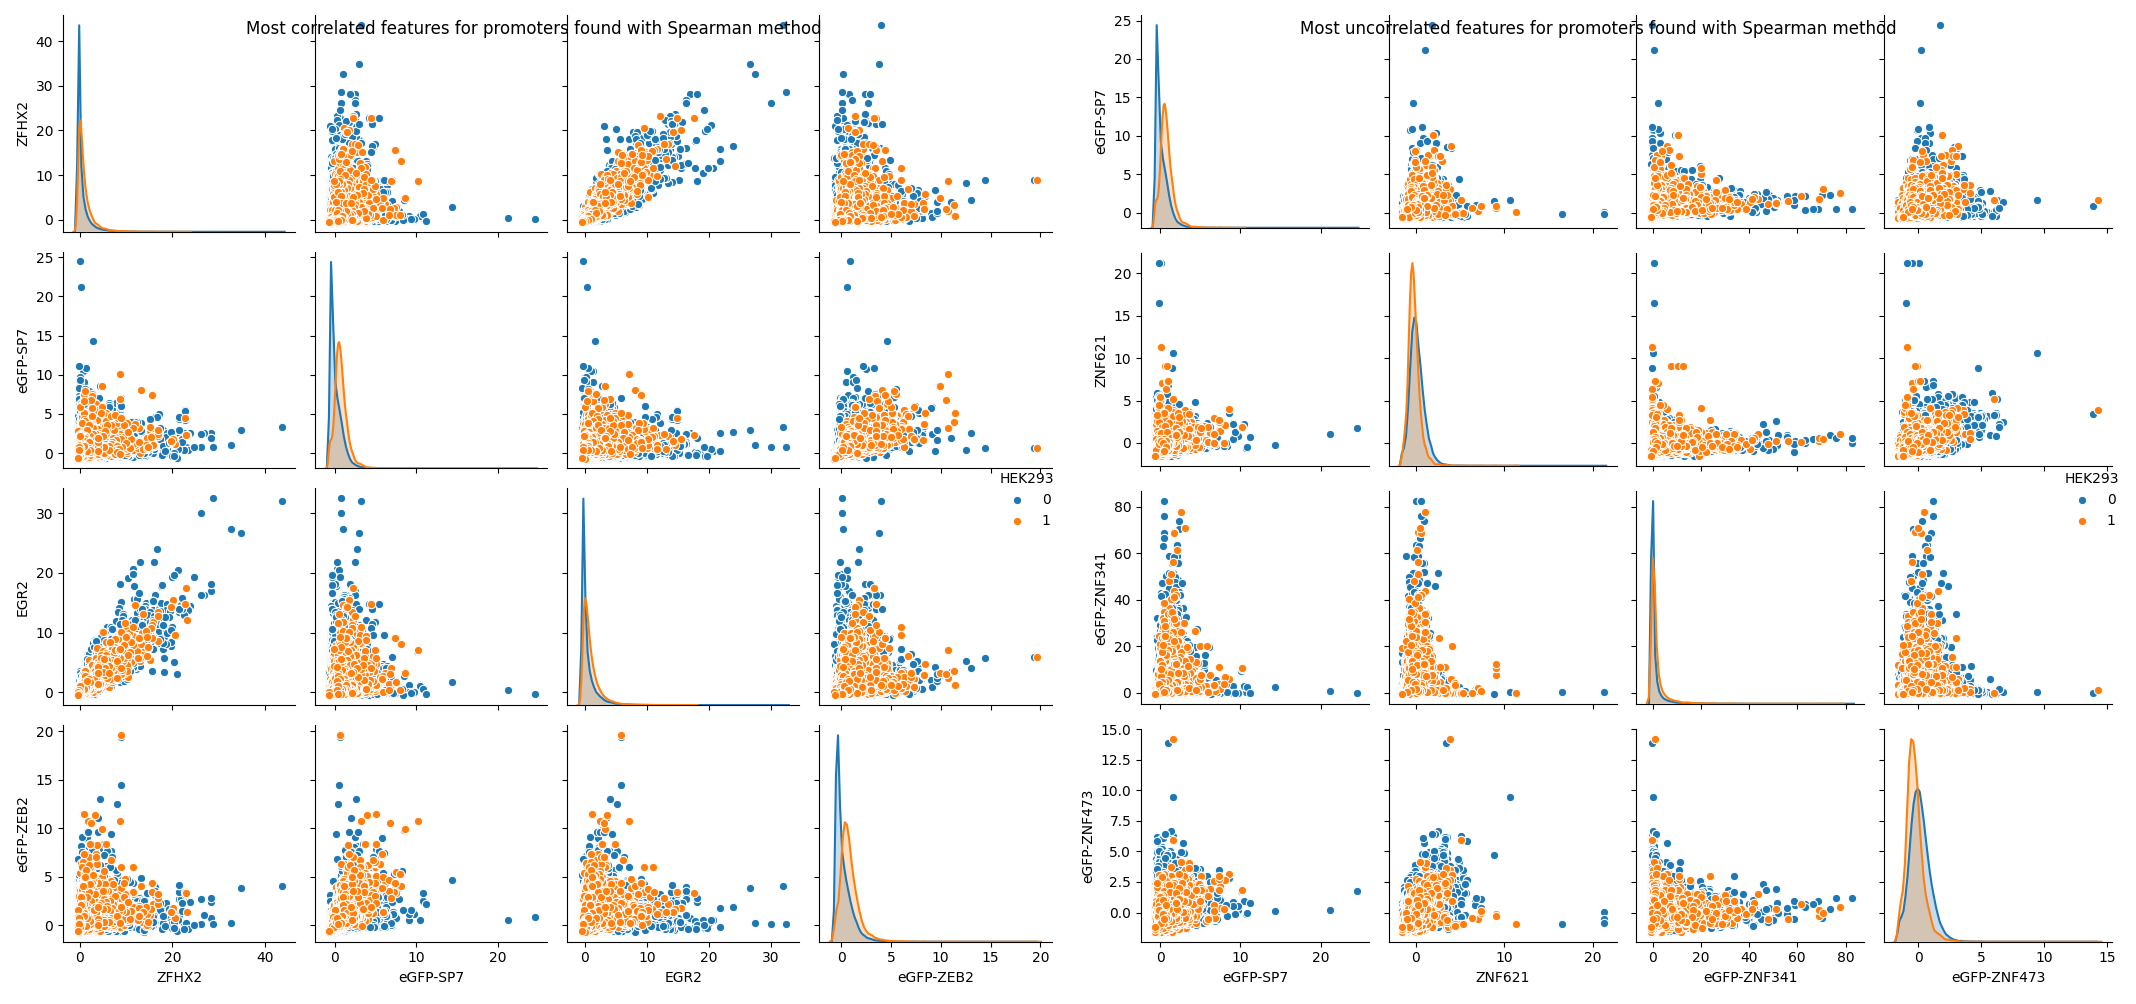
\includegraphics[width=0.98\linewidth]{../images/plot_spearman_promoters_correlated_uncorrelated.png}
\caption{Most correlated and uncorrelated feature with output for promoters found with Spearman method}
\end{figure}
\newpage
\begin{figure}[h!]
\centering
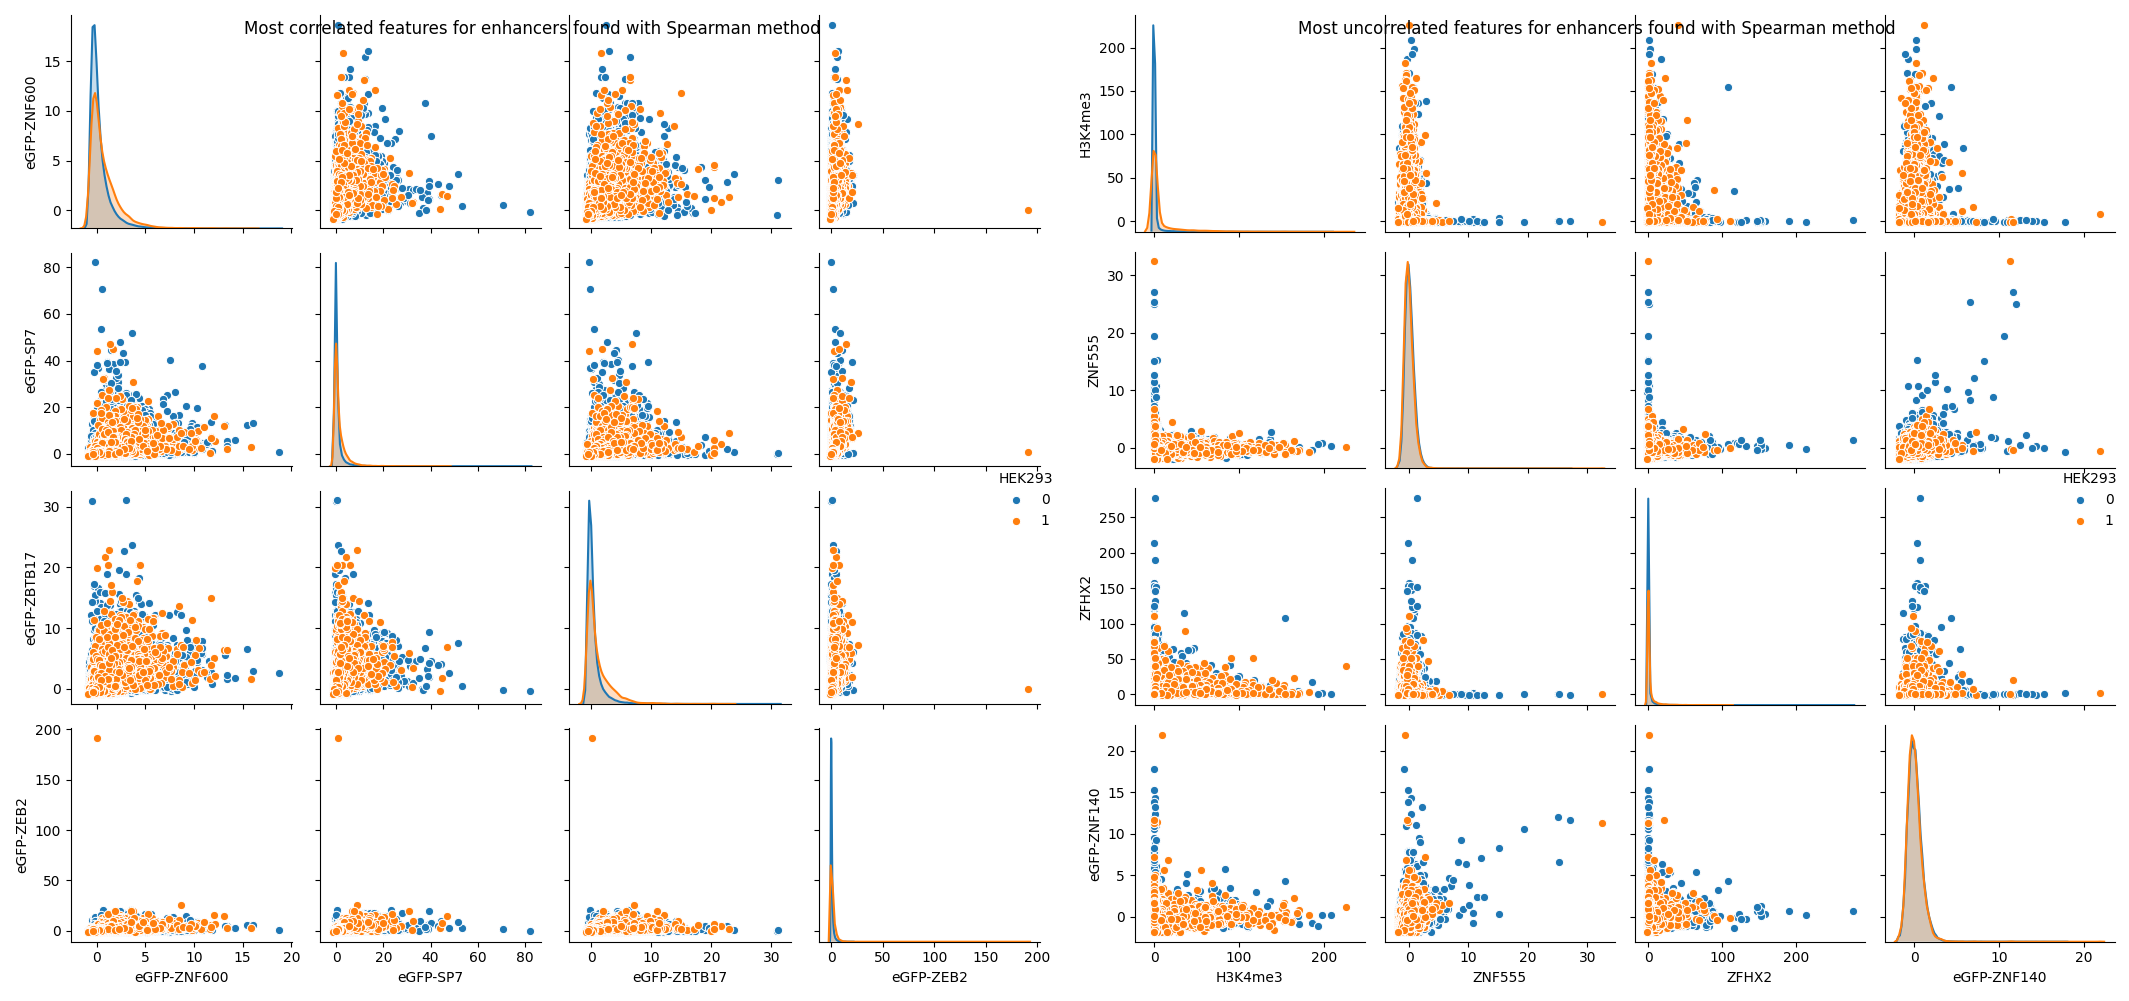
\includegraphics[width=0.98\linewidth]{../images/plot_spearman_enhancers_correlated_uncorrelated.png}
\caption{Most correlated and uncorrelated feature with output for enhancers found with Spearman method}
\end{figure}

\subsubsection{Automatic feature selection: the Boruta
method}

The feature selection is the process of finding the relevant features to
use for learning a model. Indeed the data may have some irrelevant or
redundant features, which can be removed without information loss to
make the learning process easier. Until now the feature selection
process was done using manual methods, based on the feature to feature
and the feature to output correlation. These methods are certainly
effective but there are not enough: the features are considered one or
to at a time to find a linear or non-linear correlation between the
output or another feature. Boruta, an automatic method for feature
selection, considers the features as a whole and use a specific
classification algorithm to find the irrelevant features. Boruta is a
wrapper built around the random forest algorithm, chosen because it is
relatively quick to compute and it usually can run without parameters
specification. In fact, Boruta is an ensemble method in which
classification is performed by voting of multiple decision trees, each
of them is independently developed on different samples of the training
set. The importance measure of an attribute is the loss of accuracy of
classification, caused by random permutation of this attribute values in
the various trees.

\subsection{Experiments evaluation}

After preprocessing and feature selection, the data are ready to pass to
the learning models. The holdout technique is used for testing the
models. This method consists into split the dataset in two separate
sets: the training set (used to train the leaning machine to learn) and
the test set (used to test the model performances). In this case, the
split is 80\% and 20\% for training and test set. The experiments are
executed over multiple holdouts, 50 for epigenomic data, and 3 for
sequence data, to make the models' evaluation more robust. In
particular, the StratifiedShuffleSplit of sklearn is used to make the
holdouts. This method randomly separates the training and test set
indices, preserving the percentage of samples for each class. It is set
with 42 as random\_state parameter.

The metrics used to evaluate the models are the following:

\begin{itemize}
	\item
	\textbf{accuracy:} is the ration between the correct predictions and
	the total number of samples.
	\item
	\textbf{auPRC}: the area under the precision-recall curve is a useful
	measure of success of prediction when the classes are imbalanced. The
	precision-recall curve shows the tradeoff between precision and recall
	of different thresholds. A high area under the curve represents both
	high recall and high precision, where high precision relates to a low
	false-positive rate, and high recall relates to a low false-negative
	rate. The auPRC value is between 0 and 1 and a high value denotes a
	good predictor.
	\item
	\textbf{auROC}: the area under receiver operating characteristic is a
	metric specific for binary classification tasks. It indicates the
	fraction between the true positive rate and the false-positive rates.
	Differently, form auPRC, its values are between 0.5 and 1.
\end{itemize}

Each metric is calculated for each model the final results are the mean
and the standard deviation obtained through the various holdouts. These
results are finally compared using the Wilcoxon signed-rank test with a
p\_value threshold of 0.01. It is a non-parametric statistical test to
compare hypotheses made on repeated measures.